\chapter{SBT Prototype and Cosmics Setup}\markboth{SBT Prototype and Cosmics Setup}{}\label{cosmics}

This chapter will give  an overview on the working principles of the \ac{SBT} prototype used in this thesis, and provide an introduction to the elements it is composed of.


\section{Principles of Scintillation Detection}

    Scintillation detection uses the property of luminescence of certain materials when exposed to traversing charged particles.
	The material in question can, in principle, be liquid, gaseous or solid, but different materials do show different characteristics concerning how well they scintillate under certain circumstances, making them suitable in different applications.
	Scintillators are generally put in two categories, depending on their chemical compositions - organic and inorganic.
	Both have quite different working principles, but as both the plastic and the liquid scintillator used in this experiment are organic, this next section will focus on the organic scintillation mechanism.
	In organic materials, luminescence is caused by the transition between energy states of a single molecule, as opposed to that of electrons in a crystal lattice, as would be the case for inorganic scintillators.
	For this reason, organic scintillators can exist in different physical states, and not just crystalline forms, as the chemical's molecular structure itself is conserved between the different states.

	Most organic scintillator materials contain aromatic hydrocarbon compounds.
	The electrons of the C = C bond in these molecules are delocalised, meaning they are able to 'freely' transition between energy levels.
	An electron in its ground state $S_0$ can absorb energy provided by a passing charged particle, and transition into a higher energy level - an excited state ($S_1$ and $S_2$).
	These excited states are not stable, meaning the electron will give off energy to re-enter a stable state after some amount of time.
	Usually, the energetically higher excited states are close in energy levels, and an electron will de-excite quickly to the first excited state through radiationless transitions, see also figure \ref{fig:jablonski}. It shows a Jablonski diagram of a typical organic scintillator, where the vertical distance between horizontal lines represents the energy difference between different states. The singlet excited states are denoted as $S_1$ and $S_2$, the ground state is called $S_0$.
	
%	FIGURE jablonski
	\begin{figure}
		\centering
		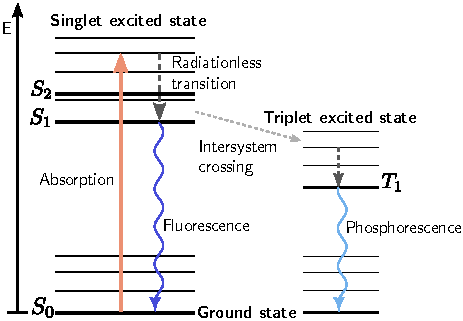
\includegraphics[width=.7\textwidth]{pictures/jablonski.pdf}
		\caption{Schematic Jablonski diagram showcasing fluorescence and phosphorescence. Based on \cite{SCINTILLATION-TORRES}.}
		\label{fig:jablonski}
	\end{figure}

	
	As pictured in the diagram, the transition to a near-ground state has a greater energetic difference than the ones between higher-lying excited states, and the excited electron will emit electromagnetic radiation in its relaxation. The time it stays in this excited state usually is of the order of a few nanoseconds. This process of relaxation via photo emission is called fluorescence \cite{SCINTILLATION-TORRES}. % and is the source of the scintillation light used to detect an incoming particle in both the \ac{SBT} detectors as well as the cosmics setup.
	
	Fluorescence however is not the only process in which light can be produced through excitement of an electron. For most molecules, the electrons ground state is a singlet state, and they usually get excited into a higher lying singlet state as well. There is however the possibility of the electron experiencing intersystem crossing into an excited triplet state, called $T_1$ in figure \ref{fig:jablonski}, and transitioning back to the ground state from there. This process is called phosphorescence and influences the overall luminescence of a chemical, as it lowers the amount of fluorescence light emitted in a given time: The process of intersystem crossing is suppressed and therefore carries out over a time span of microseconds, which is significantly slower than fluorescence.
	
	While the amount of scintillation photons produced depends on the incoming particles' energy, it is not a fixed value for a set of circumstances. The average energy deposited by a heavy charged particle such as a muon in a medium is generally described by the Bethe-Bloch-Formula \cite{SCINTILLATION-TORRES} (barring some corrections), however as the interaction itself is still a scattering process, the actual number of photons produced underlies statistical fluctuations. 
	These statistical fluctuations are dependent on the geometry of the scintillation detector, which has to be studied for each detector individually \cite{GEOMETRIES}.
	
	
	
	
%	The plastic scintillators used for positional data acquisition in the cosmics setup at \ac{HU} Berlin are general purpose \ac{PS}, type NE-110, produced by Eljen Technology. They emit light mainly on a spectrum of 420 to \SI{480}{\nano\meter} \cite{ELJEN-site}, which lies in the visible spectrum and does not need to be shifted to be easily detected.


\section{Photodetection} \label{photodetectors}

The \ac{SBT} prototype uses two different types of photodetectors to detect scintillation light caused by charged particles. \acsp{SiPM} are used inside the \ac{LS} box, \acsp{PMT} are attached to the plastic scintillators outside the detector box.


\subsection{Silicon Photomultipliers}  

Silicon photomultipliers are a nowadays relatively common way to detect photons, as they are compact, robust and less expensive than other detectors, while offering a high detection efficiency and time resolution.

Most \acsp{SiPM} are made up of many \acfp{SPAD}, the so-called pixels, which are arranged in a matrix structure. Each \ac{SPAD} is a diode, operated under reverse bias. An incident photon will create an electron-hole pair in the diode's semiconductor layer via the photoelectric effect \cite{HAMAMATSU-SIPM}. The generated charge, amplified through avalanches caused by the bias voltage, is then read-out as a current.

\begin{figure}
	\centering
	\begin{subfigure}{.4\textwidth}
		\centering
		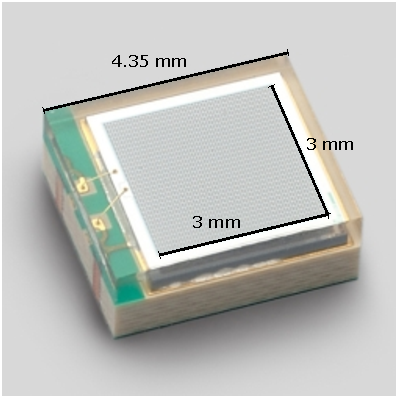
\includegraphics[width=\textwidth]{pictures/sipm.pdf}
		\caption{S13360-3075PE \ac{SiPM} produced by Hamamatsu. Photo adapted from \cite{HAMAMATSU-cell}.}
	\end{subfigure} \hfill%
	\begin{subfigure}{.5\textwidth}
		\centering
		\includegraphics[width=.9\textwidth]{pictures/sipm-array.pdf}
		\caption{40 \acsp{SiPM} arranged on a \ac{PCB}.}
	\end{subfigure} 
	\caption{Photos of Hamamatsu \acsp{SiPM}.}
	\label{fig:sipm-photos}
\end{figure}





\subsection{Photomultiplier Tubes}
%\ac{PMT}


The cosmics setup additionally utilises four \acsp{PMT} for light detection.
%\todo{high voltage?}

%	FIGURE photomultiplier tube
\begin{figure}[h]
	\centering
	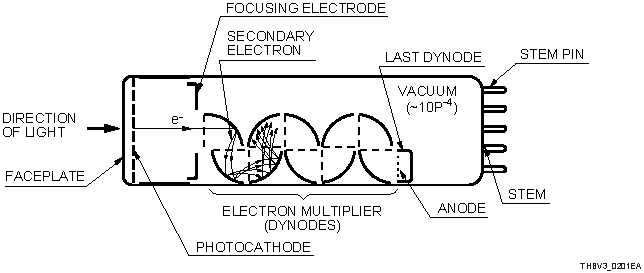
\includegraphics[width=.8\textwidth]{pictures/photomultiplier.pdf}
	\caption{Schematic of a \acl{PMT}. An electron emitted from the photocathode by incident light gets 'multiplied' in the dynodes by knocking additional electrons loose in the material, which then get accelerated towards the next dynode. The tube is evacuated to guarantee unhindered flight for the electrons. Image taken from \cite{HAMAMATSU-PMT}.}
	\label{fig:photomultiplier}
\end{figure}


The general structure of a \acl{PMT} can be viewed in \ref{fig:photomultiplier}. As a photon enters the tube through the input window, called the faceplate, it can excite an electron in the photocathode, given the photon had the minimum required energy required to ionise the cathode material. This electron, now emitted into the vacuum of the tube via the photoelectric effect, will be accelerated by the electric field between the cathode and the first electrode, the focussing electrode, and directed towards the electron multipliers, called dynodes. As the accelerated electron has more energy now than when it started, upon striking the surface of a dynode, some number of secondary electrons are emitted from the dynode by the collision. These secondary electrons are then once again accelerated towards another dynode, and the process gets repeated. 
This means that a single photon could, after some stages of multiplying, cause a signal of several measurable electrons in the anode, where all secondary electrons are collected and output to an external circuit in the form of a current \cite{HAMAMATSU-PMT}.
The strength of the current amplification caused by the \ac{PMT} is dependent on the number and layout of dynodes in the \ac{PMT}, as well as the voltage applied to accelerate the electrons between them \cite{HAMAMATSU-PMT}. These factors are also what mainly determines the response time of a \ac{PMT} as they affect the speed at which electrons transit between cathode, dynodes, and anode \cite{HAMAMATSU-PMT}.




\section{Wavelength-shifting Optical Module}

	As it is very expensive to cover a whole detector box with photosensors, the scintillation light produced in the box filled with \ac{LS} needs to be gathered and transported toward photodetectors to be readout and used in analysis. For this, the \ac{LS} prototype uses a so-called \ac{WOM}, which are also going to be implemented into the \ac{SBT}. The \ac{WOM}-setup consists of a \ac{PMMA} tube coated with \ac{WLS} paint.
	

	
	The emission spectrum of the liquid scintillator used in the \ac{LS} prototype is shown in figure \ref{fig:absorption-emission}. It peaks around 350 to \SI{400}{\nano\meter}, which lies in the ultraviolet range. Most common photodetectors that are suitable for the experiment however are most efficient in the visible spectrum \cite{SPECTRAL-SEMICONDUCTOR}. This is the reason the \ac{WOM} tube is coated in the \ac{WLS} paint: The paint absorbs light in the spectrum of 300 to \SI{400}{\nano\meter}, and re-emits light at a higher wavelength, peaking around \SI{420}{\nano\meter} (see figure \ref{fig:absorption-emission}). This emission range is also the reason for the blue sheen the \ac{WOM} shows in photos like figure \ref{fig:WOM-tube}: The wavelength-shifted emission light has a wavelength that humans call blue.
	
	%    FIGURE absorption emission LAB and WLS
	\begin{figure}[h]
		\centering
		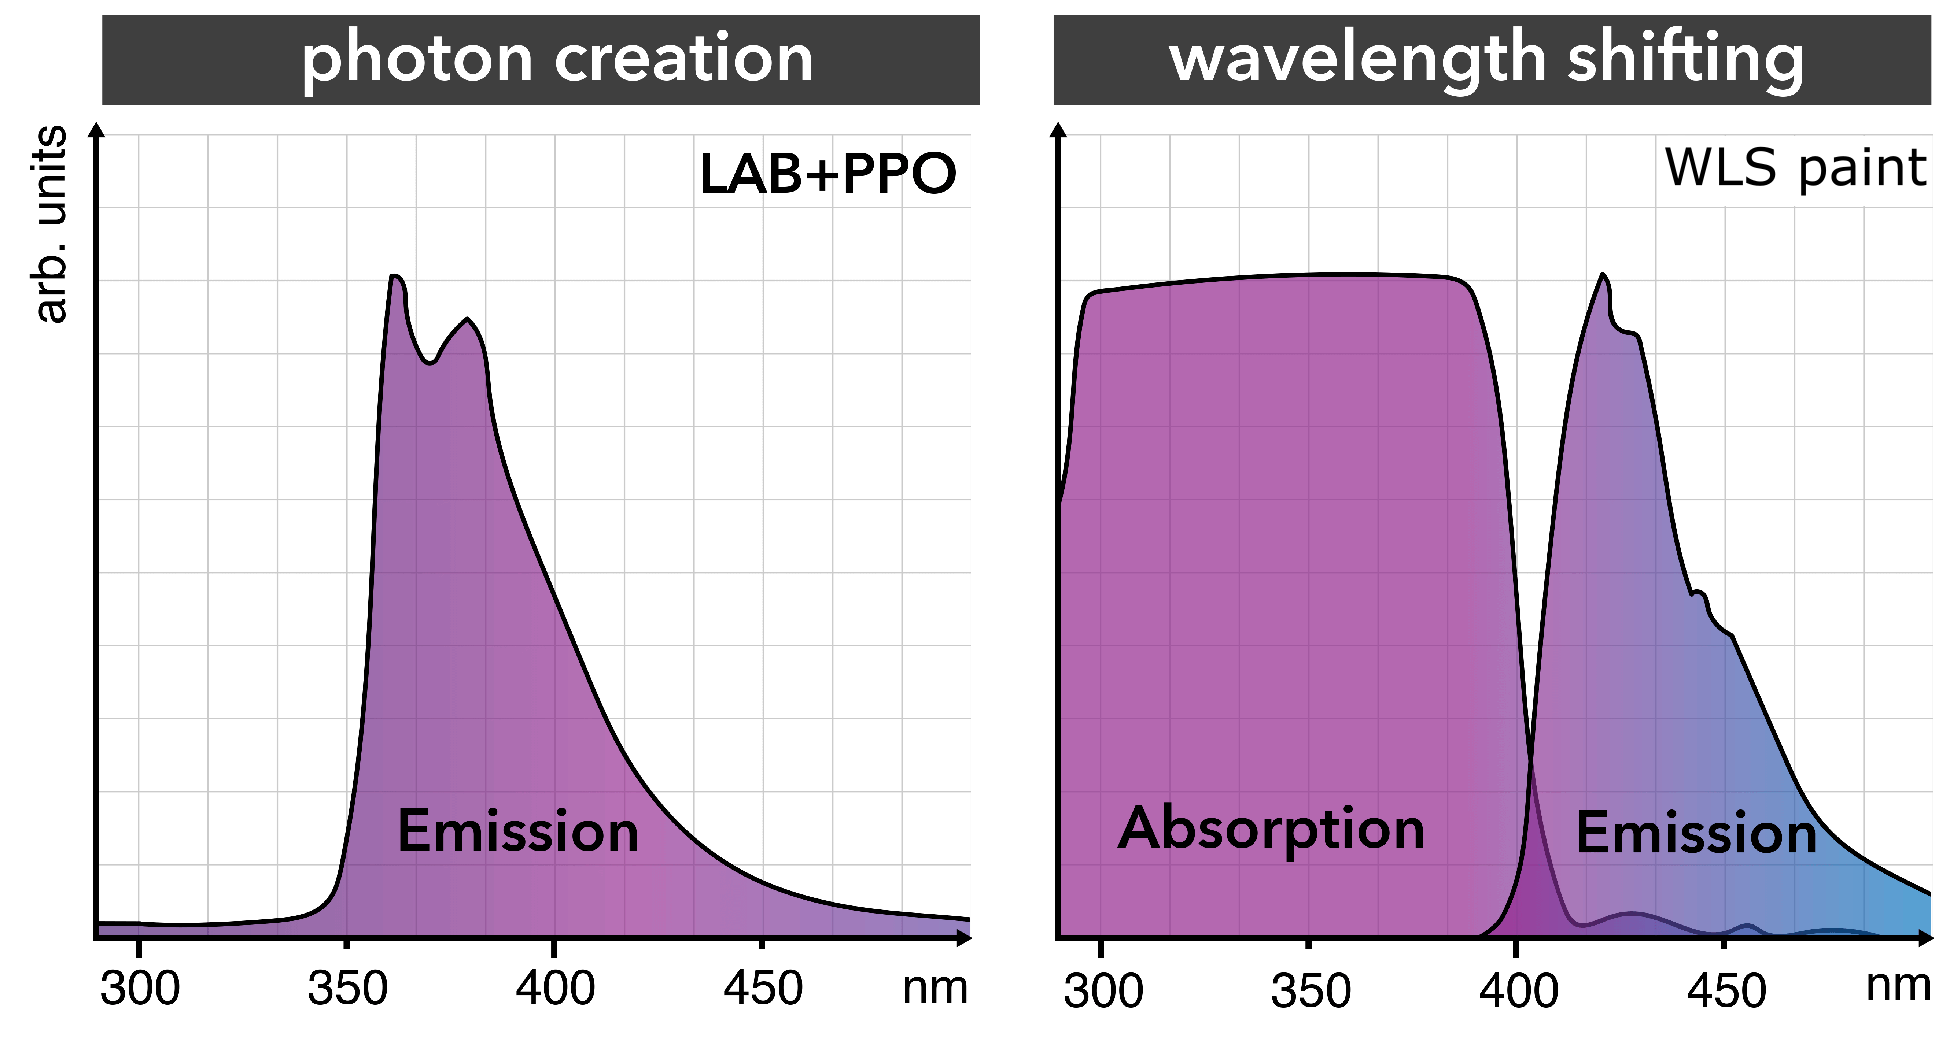
\includegraphics[width=.7\linewidth]{pictures/absorption-emission.png}
		\caption{Emission spectrum of \ac{LAB}+\ac{PPO} liquid scintillator used in the prototype (left), absorption and emission spectrum of \ac{WLS} paint that's coated onto the \ac{WOM}. The paint absorbs photons emitted by the \ac{LS}, and re-emits photons with a higher wavelength, shifting them from UV to visible spectrum. Diagram not true to detail. Made by Jan Zimmermann \cite{ZIMMERMANN}, based on \cite{EHLERT}.}
		\label{fig:absorption-emission}
	\end{figure}
	
	After being absorbed and re-emitted by the \ac{WLS} coat, the scintillation photons travel inside the \ac{WOM} tube. 

	In the tube, the re-emitted scintillation light is transported towards the \acsp{SiPM}, which are located on the end of the tube, via total reflection: The tube and the \ac{LS} are not touching each other, as the \ac{WOM} tube is inserted into a vessel, also made of \ac{PMMA}.
	
	
	
	%    FIGURE WOM inside PMMA vessel
	
	\begin{figure}[h]
		\centering
		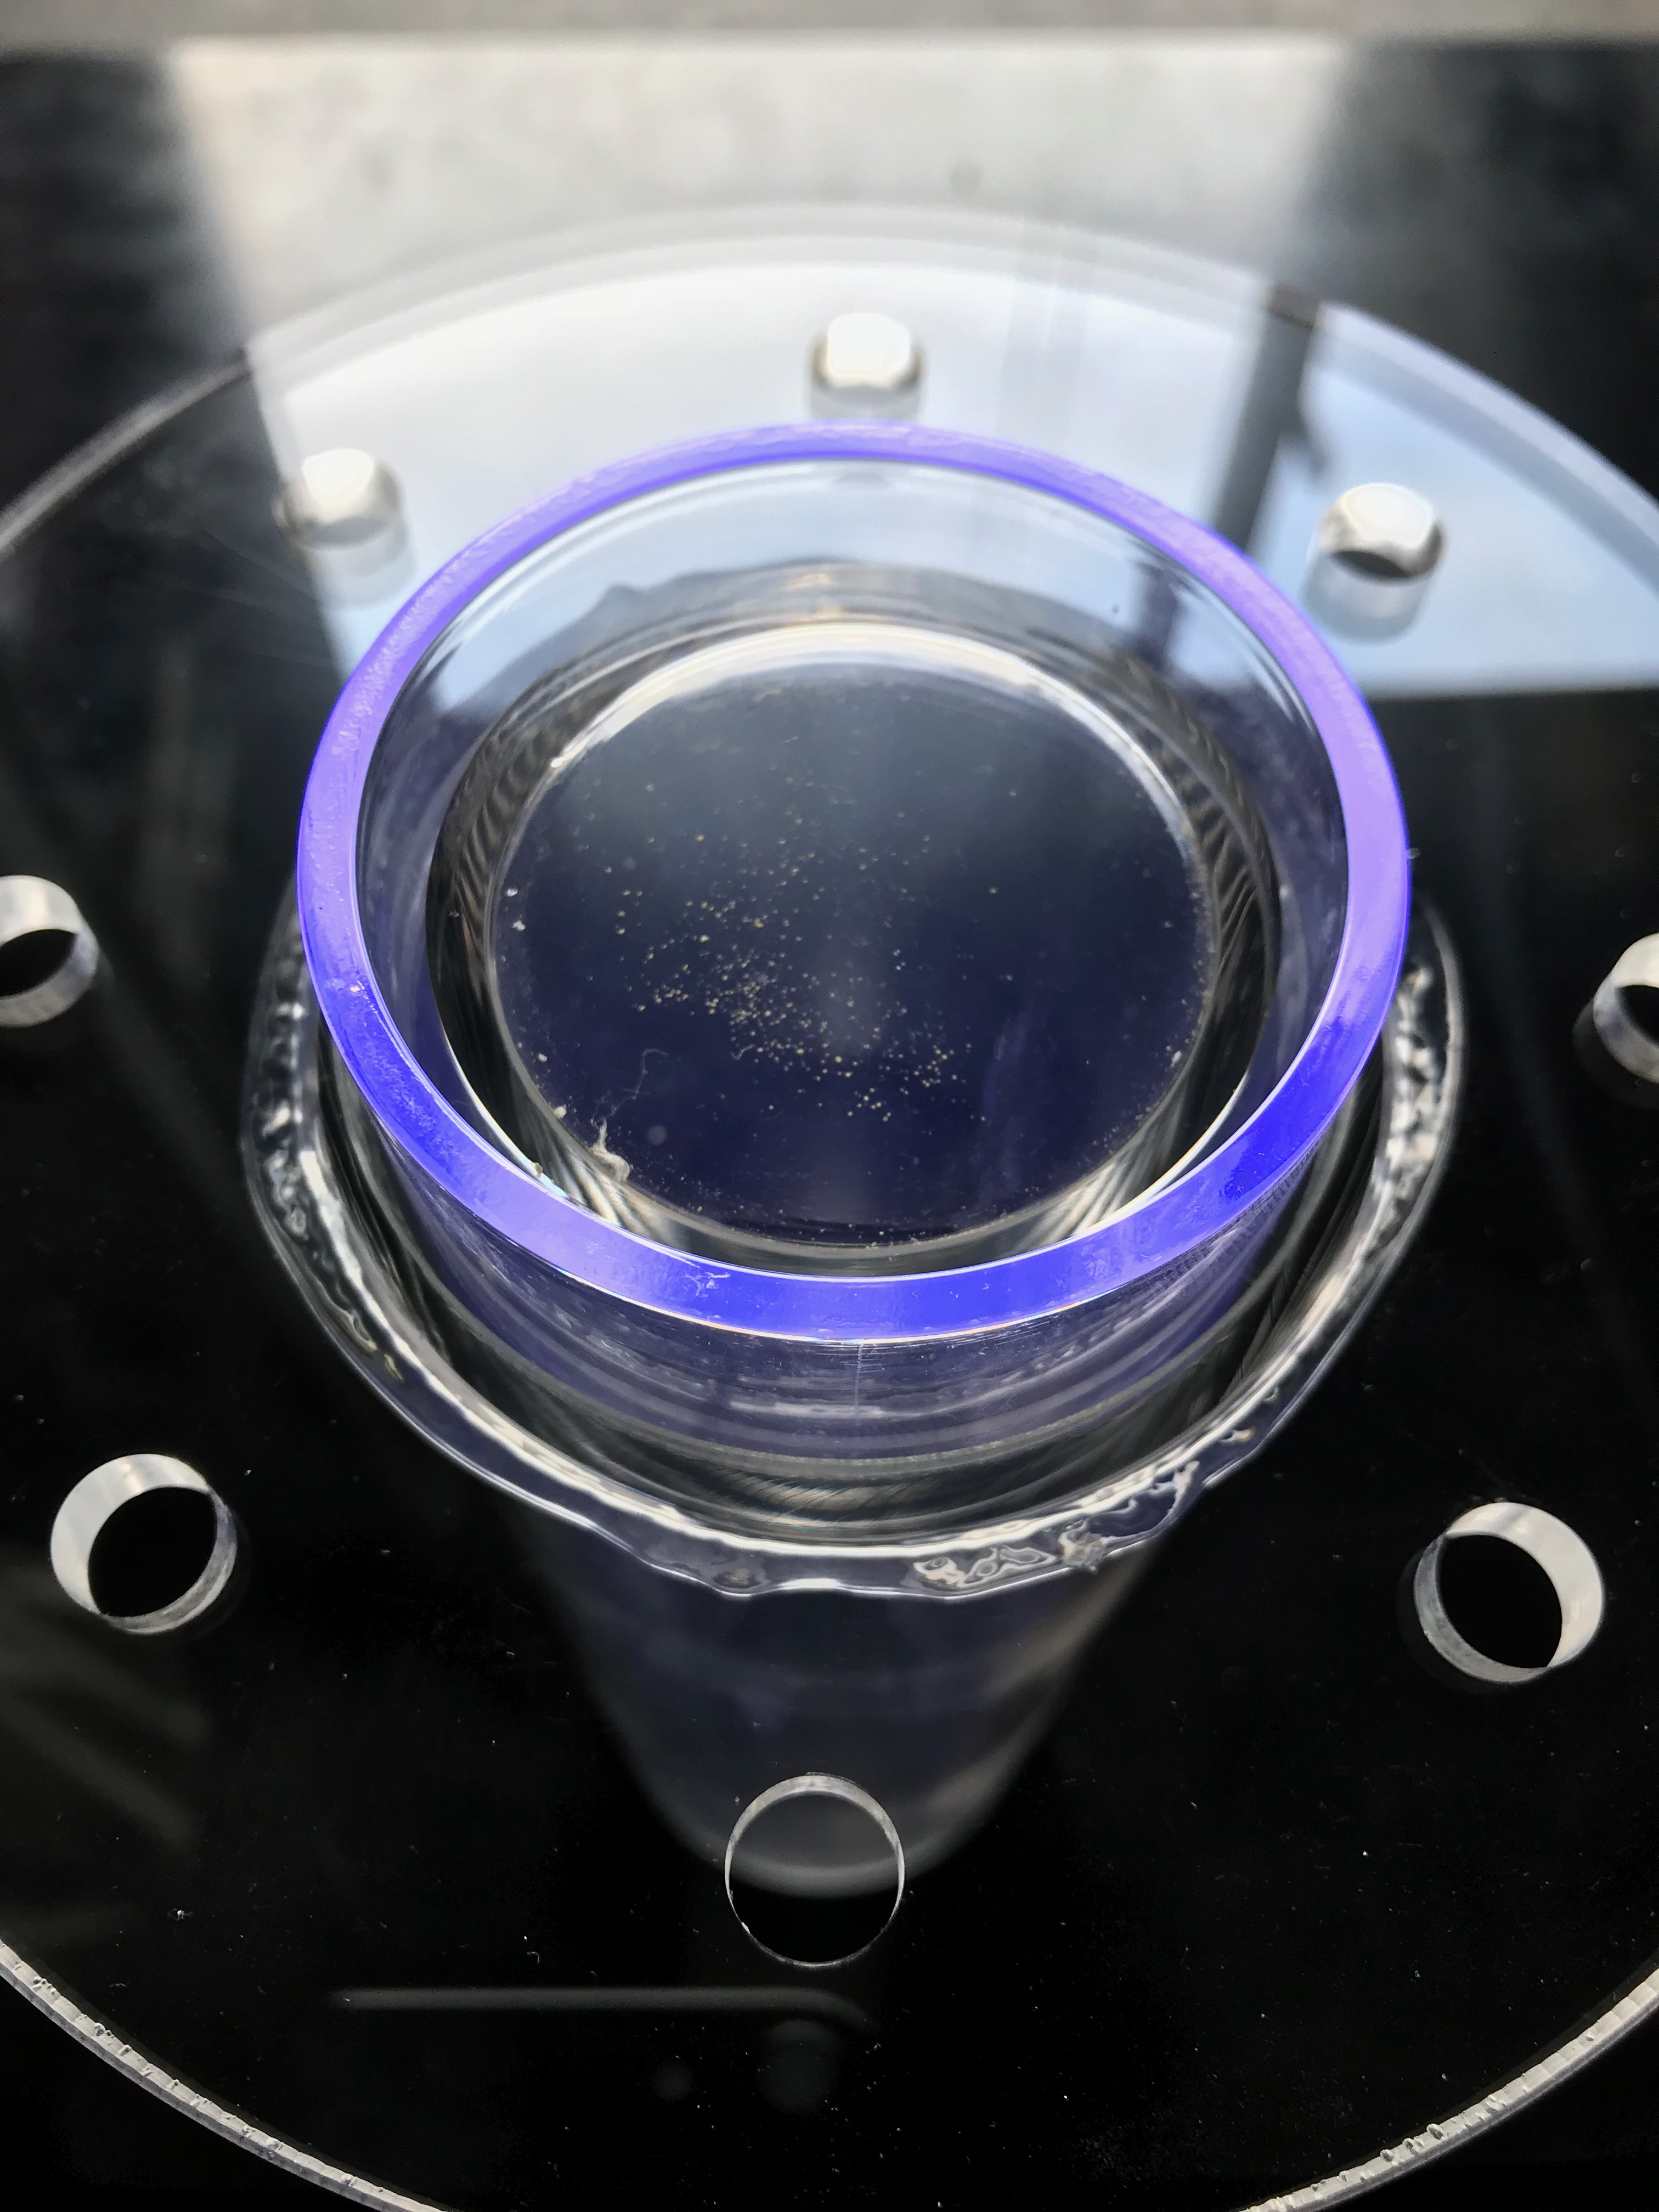
\includegraphics[width=.5\textwidth]{pictures/WOM_Vessel_TB18_top.jpeg}
		\caption{\ac{WOM} tube, coated with \ac{WLS} paint, inside \ac{PMMA} vessel. Photo was taken at a test experiment at \ac{DESY} in 2018.}
		\label{fig:WOM-tube}
	\end{figure}
	
	As illustrated in figure \ref{fig:wom-principle}, the vessel and the tube also have some space between them, filled with air. As such, one can calculate the critical angle for total internal reflection $\theta_{crit}$ on the surface of the tube according to Snell's law \cite{ZINTH}, using the refraction indices of air and the tube:
	
	\begin{align}
		\theta_{crit} = \arcsin(\frac{n_{air}}{n_{tube}}) \simeq \arcsin(\frac{1}{1.5}) = \SI{41.8}{\degree}
	\end{align}

	\begin{figure}[h]
		\centering
		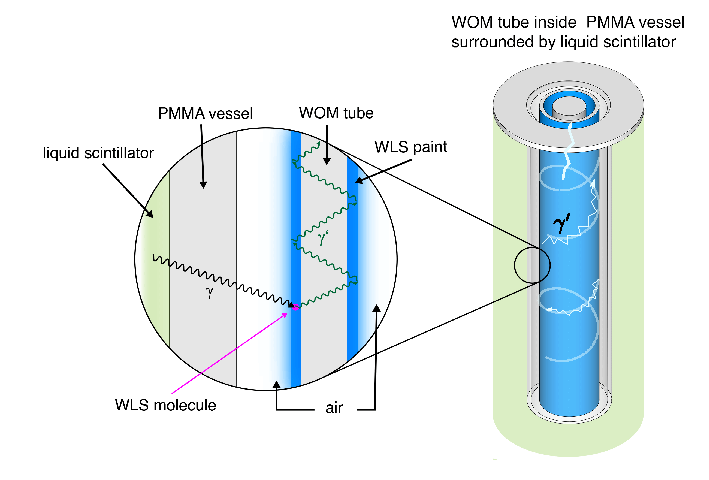
\includegraphics[width=.8\textwidth]{pictures/wom-principle.pdf}
		\caption{Illustration of the \ac{WOM} principle, showing, on the right-hand side, a \ac{WOM} tube (blue) inside a \ac{PMMA} vessel (grey), inside the liquid scintillator (green). The close-up (left) shows a scintillation photon $\gamma$ absorbed and re-emitted by the \ac{WLS} paint (blue), resulting in a photon $\gamma'$ that is emitted isotropically into the \ac{WOM} tube (grey). At the surfaces of the tube with air, the photon experiences total reflection, and is redirected back into the tube. This reflection occurs multiple times, until the photon reaches the end of the tube, where \acsp{SiPM} are located (not shown). Illustration adapted from \cite{ZIMMERMANN}.}
		\label{fig:wom-principle}
	\end{figure}

	Photons meeting the \ac{WOM}'s surface at this or greater angles will be getting reflected off the walls again and again. As there is no preferred direction to the re-emission of photons from the \ac{WLS} paint, the photons are not going to be transported to the end of the tube, where the photodetectors are located, on the shortest path possible. It is more likely that they travel in some sort of spiral along the cylindrical \ac{WOM} tube \cite{HANEL}, as indicated in figure \ref{fig:wom-principle} on the right-hand side. This effect is part of the challenge of using the \ac{WOM} setup and determining positional data from the photodetectors' signal: Where a photon created somewhere in the \ac{LS} ends up being detected at the end of the \ac{WOM} tube is greatly dependent on the tube and its optical coupling to the photodetectors, rather than just the location of the initial scintillation light.
	
	The connection between \ac{WOM} tube and the circular array of silicon based photodetectors is given by an optical gel. Both the \ac{PCB}, on which the \acsp{SiPM} are mounted, and the \ac{WOM} tube have an outer diameter of \SI{6}{\centi\meter} and width of \SI{3}{\milli\meter}, meaning the \acsp{SiPM} cover the entire \ac{WOM} cross section's surface area. 
%	 To ensure the \ac{PCB} is connected to the tube as statically as possible, minimising the variation in optical coupling, the whole setup is fixated to the detector box.

    
    
    % Neglecting any transporting losses or imperfections in the total reflection, this critical angle would suggest that $1 - \nicefrac{41.8}{180} \simeq \SI{76.8}{\percent}$ of incoming photons are reflected off of the surface of the tube. 
    
    
    
    

    

%    As is already implied in the Jablonski diagram in the previous section, the wavelength of scintillation photons produced in the fluorescence process depends on which state transition took place. As such, an organic scintillator actually scintillates on a certain spectrum of light, which is not necessarily easily detectable with the available photodetectors. All scintillators however emit light with the same or higher wavelength than they have previously absorbed - this is evident in the diagram as well as clear when considering energy conservation.
    

    
    
    




\section{The SBT Prototype}
%general introduction to the experiment

%To study the incidence location-dependent behaviour of a \ac{PMMA} vessel with a mounted PCB, an \ac{SBT} cell-like prototype was used. It is pictured in figure \ref{fig:cosmics-photo}.
%  combined with a set of two plastic scintillators - the cosmics setup (figure \ref{fig:cosmics-photo}).
In this thesis, cosmic muons were used to study the detector response of an \ac{SBT} prototype, and to which degree this response can be used to infer a muon's crossing position.
% cause scintillation light in both materials. The signals measured by the photodetectors attached to the respective scintillators are then readout and compared.

\begin{figure}[h]
	\centering
	\includegraphics[width=.6\textwidth]{pictures/cosmics-photo.pdf}
	\caption{Photo of the cosmics setup in the laboratory at \ac{HU} Berlin.}
	\label{fig:cosmics-photo}
\end{figure}

The prototype, pictured in figure \ref{fig:cosmics-photo}, consists of a box of stainless steel, with dimensions \break \SI{50.4 x 50.4 x 25}{\centi\meter}, that holds a liquid scintillator made of \ac{LAB} and \ac{PPO}. The \ac{PPO} is solved in the \ac{LAB} in a concentration of \SI{2}{\gram\per\liter}.
The steel box has wall thicknesses of \SI{1}{\centi\meter} on the sides, \SI{2}{\centi\meter} on the bottom, and \SI{0.5}{\centi\meter} on the top wall, resulting in \SI{52.7}{\liter} of \ac{LS}.
The decision to use this liquid scintillator material was made for several reasons: Liquid scintillators provide high detection efficiency as well as good area coverage, while being less expensive than solid counterparts. The scintillator material of \ac{PPO} was chosen because, compared to other materials considered, it showed the lowest response times to events \cite{ZIMMERMANN}. The solvent \ac{LAB} was preferred over others as it is cost efficient \cite{SHIP-DESIGN-2019} and raised fewer safety concerns compared to other materials \cite{ZIMMERMANN}.
% whose pressure is controlled by a valve located on top of the box.
Several holes have been worked into the steel, each of them to the size that a \ac{PMMA} vessel containing a \ac{WOM} could be inserted. However in this experiment, only the central position was used, while all other holes as well as junctions were sealed to prevent light leakage.
A photo of a \ac{WOM} tube inside a vessel can be seen in figure \ref{fig:WOM-tube} - both are about \SI{23}{\centi\meter} long and \SI{3}{\milli\meter} thick. The vessel containing the \ac{WOM} tube is about \SI{70}{\milli\meter} in diameter.

% Placed above and below the detector box is a \ac{PS} respectively, used to determine the locations of muon events.

The \acsp{SiPM} used in the cosmics setup, as well as in previous \ac{SBT} cell prototypes, are of the type S13360-3075PE, produced by the manufacturer Hamamatsu \cite{HAMAMATSU}, operated at a bias voltage of \SI{58}{\volt}. They have a breakdown voltage of \SI{53}{\volt} \cite{HAMAMATSU}, meaning the overvoltage applied is $\SI{58}{\volt} - \SI{53}{\volt} = \SI{5}{\volt}$. There is 40 \acsp{SiPM} used to detect scintillation light gathered in the detection box, aggregated in groups of five and arranged in a circle on a \ac{PCB} as depicted in figure \ref{fig:sipm-photos}. Each \ac{SiPM} covers an area of \SI{3x3}{\milli\meter}. The \ac{PCB} has a diameter of \SI{6}{\centi\meter}, to match the outer edge of the \ac{WOM} tube. As mentioned above, the photodetectors and the \ac{WOM} tube are optically coupled using the optical gel Baysilone \cite{ZACHARIAS}.





%This chapter aims to explain the working principles of scintillation detection and give insight into the function of the main components of the cosmics setup, illustrated in the schematic in \ref{fig:cosmics-setup}. 

%\subsection{Readout Electronics}

	
	

\section{The Cosmics Setup}

	To determine the position of cosmic muons crossing the prototype detector, a set of two plastic scintillators were used in the cosmics setup. A schematic of this can be viewed in \ref{fig:cosmics-setup}.
	Scintillation light produced in those was collected and detected by four \acsp{PMT}. They're of the type XP2008, manufactured by Koninklijke Philips N.V., and mounted on either side of the two plastic scintillators used to locate muon events.
 	Cosmic muons crossing the plastic scintillators and the detector box cause scintillation light in both materials. The plastic scintillators are general purpose \ac{PS}, type NE-110, produced by Eljen Technology. They emit light mainly on a spectrum of 420 to \SI{480}{\nano\meter} \cite{ELJEN-site}, which lies in the visible spectrum and does not need to be wavelength-shifted to be easily detected.


\begin{figure}
	\centering
	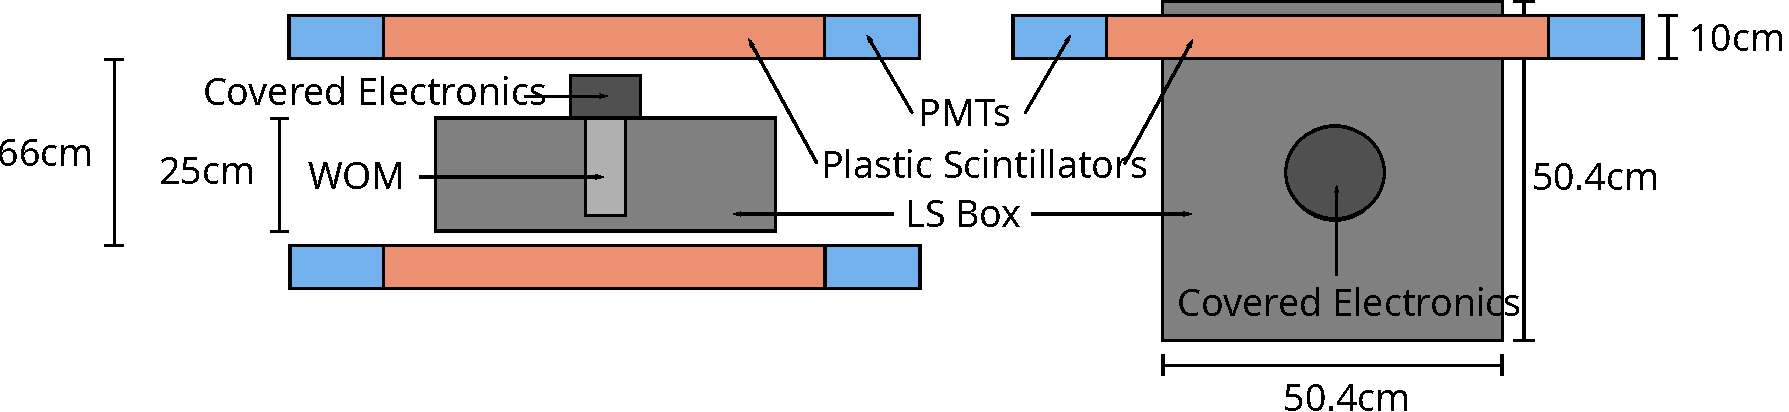
\includegraphics[width=\textwidth]{pictures/cosmics.pdf}
	%		\todo[inline]{maybe measurements PS?}
	\caption{Schematic of cosmics setup as seen from the front (left picture) and top (right picture). The liquid scintillator box (grey), containing the \ac{WOM} tube (light-grey), on top of which the readout electronics are located, covered by a light tight seal (dark-grey). Above and beneath the box, a plastic scintillator (orange), connected to two \acsp{PMT} (blue) each.}
	\label{fig:cosmics-setup}
\end{figure}

The electronic signals from the 40 \ac{SiPM} on the \ac{PCB} are pre-processed by an eMUSIC Miniboard v2, manufactured by Scientifica \cite{scientifica}. The eMUSIC board has 8 analogue input channels, to which the \acs{SiPM} are connected in groups of 5. The five signals from the individual \acsp{SiPM} gets summed into a singular waveform this way. The eMUSIC board, which amplifies these signals, is powered by a low voltage of \SI{6.5}{\volt}, but is also connected to the high-voltage source used to power the \acsp{SiPM} on the \ac{PCB}.
The eMUSIC board attached to the \ac{PCB} can be seen in figure \ref{fig:electronics}.



\begin{figure}[h]
	\centering
	\begin{subfigure}{.4\textwidth}
		\centering
		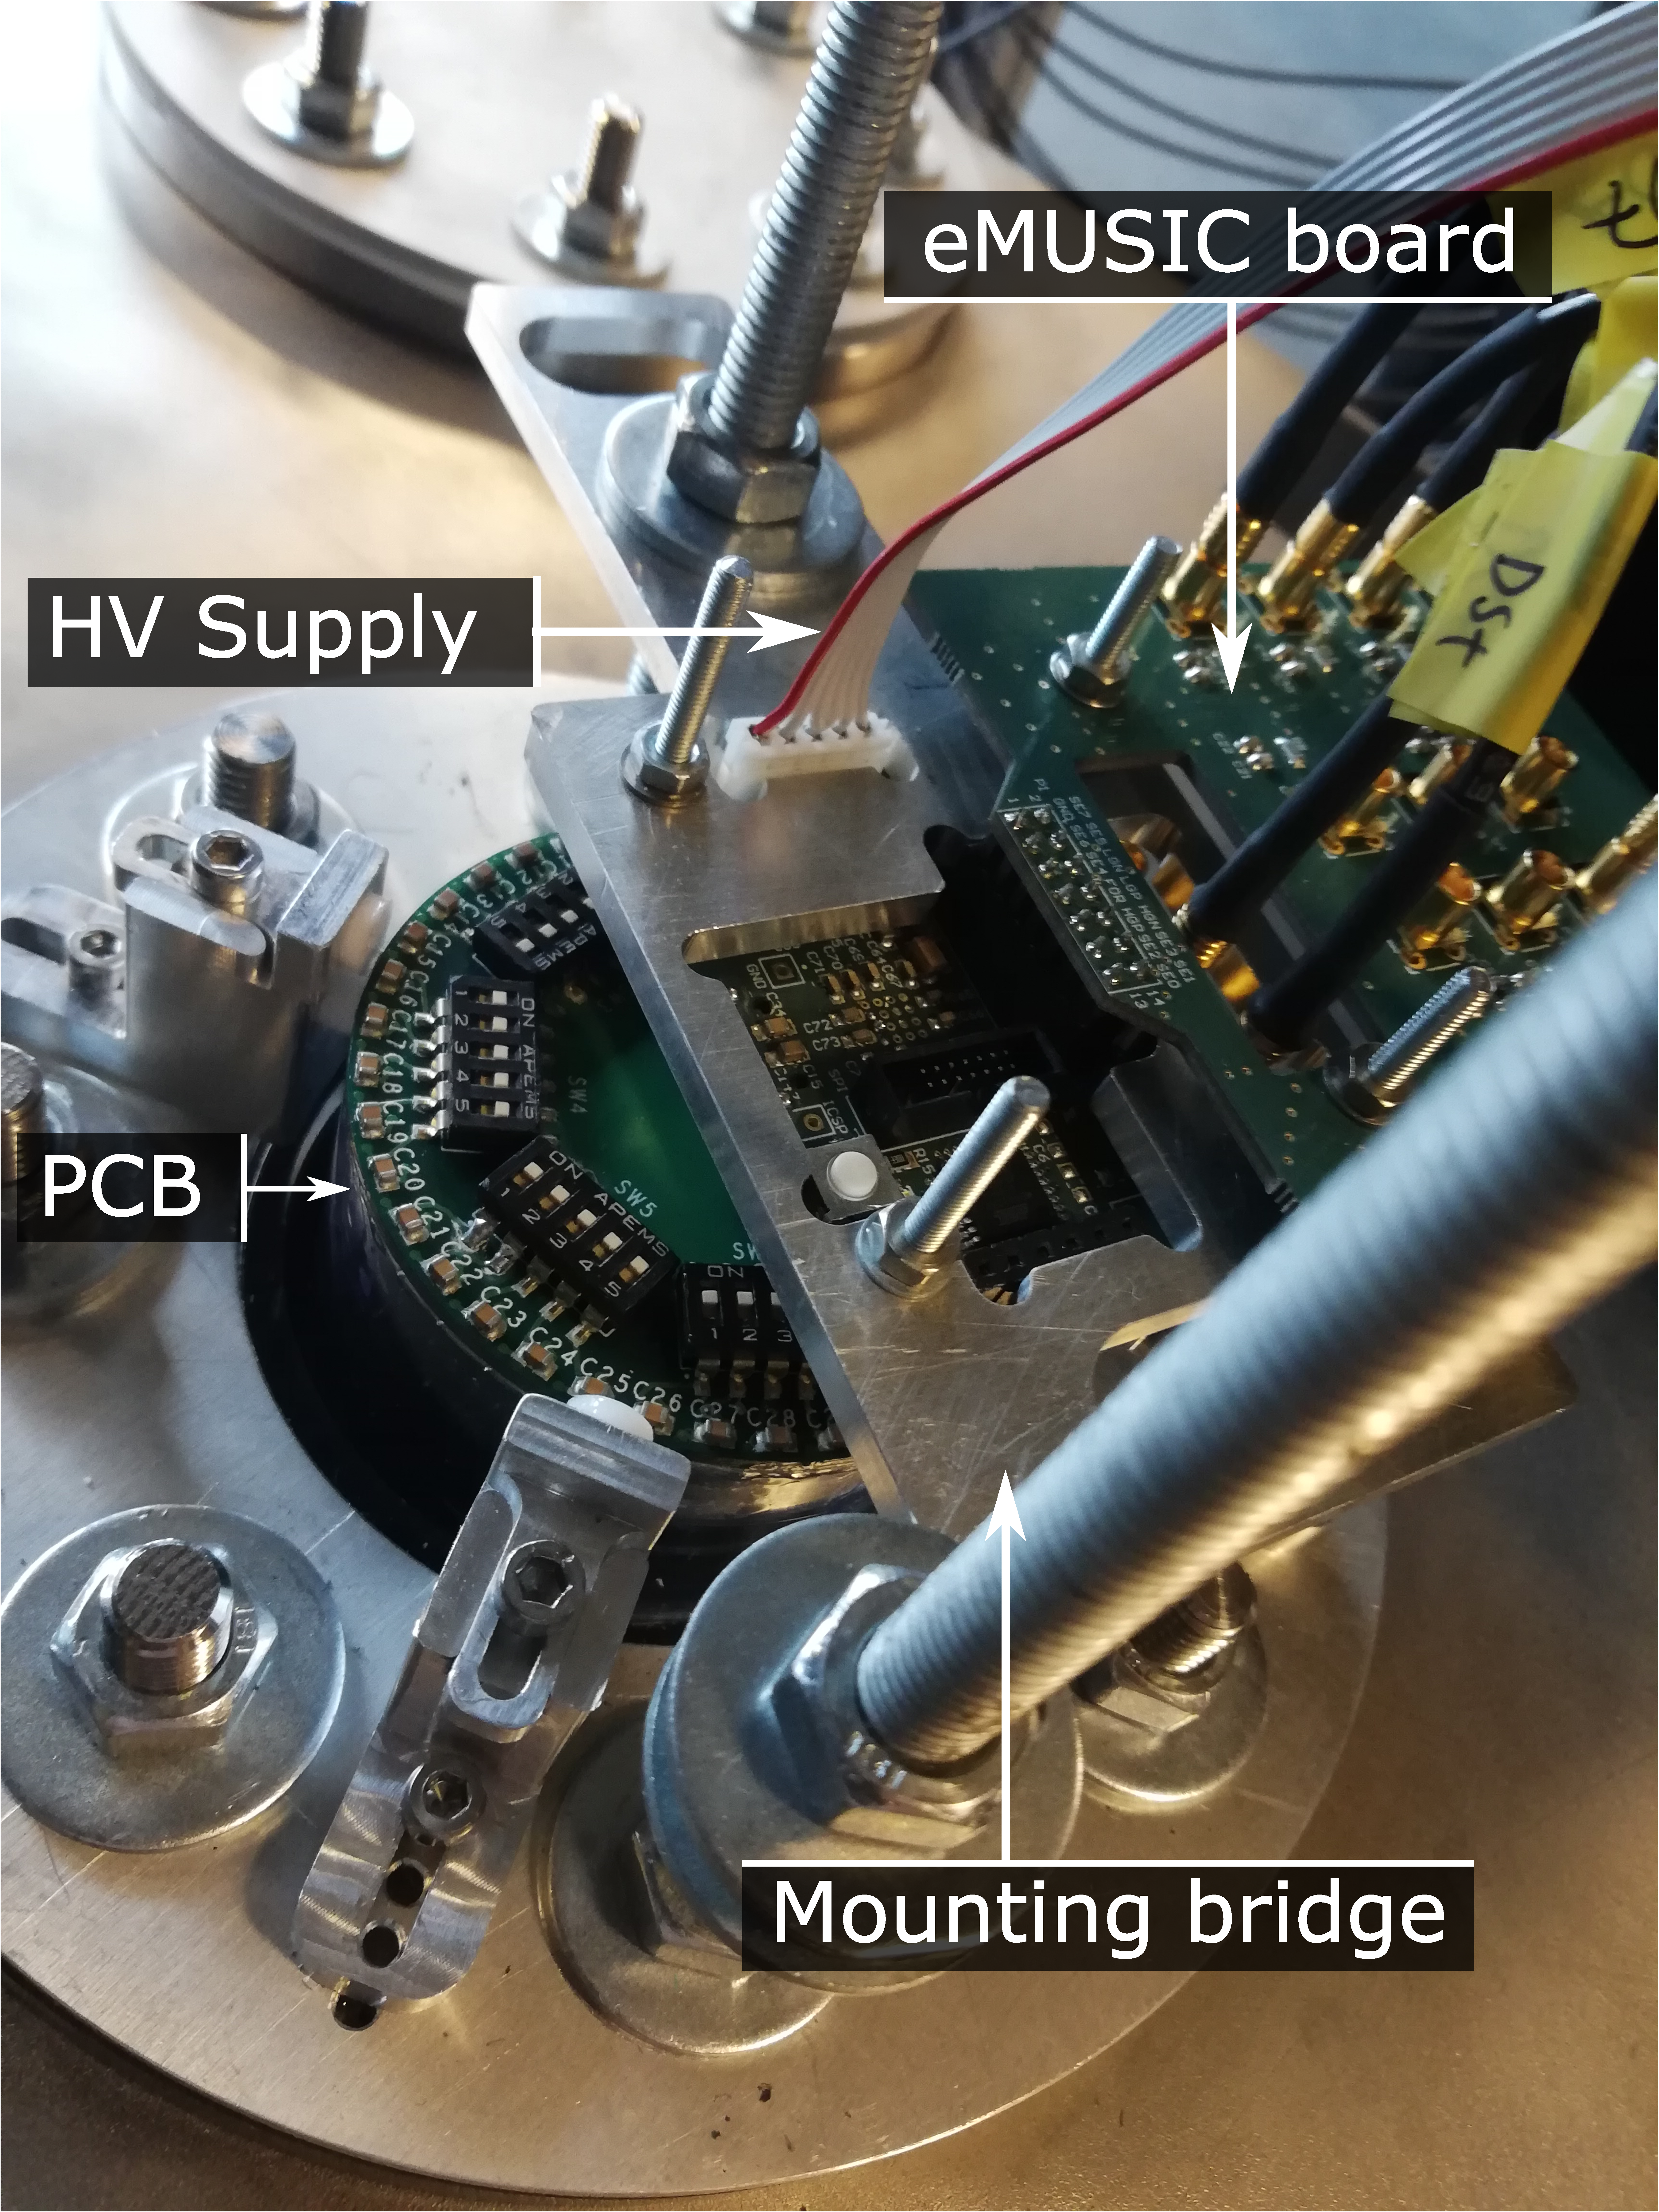
\includegraphics[width=\textwidth]{pictures/electronics-voltage.pdf}
		\caption{}
	\end{subfigure}\hfill%
	\begin{subfigure}{.5\textwidth}
		\centering
		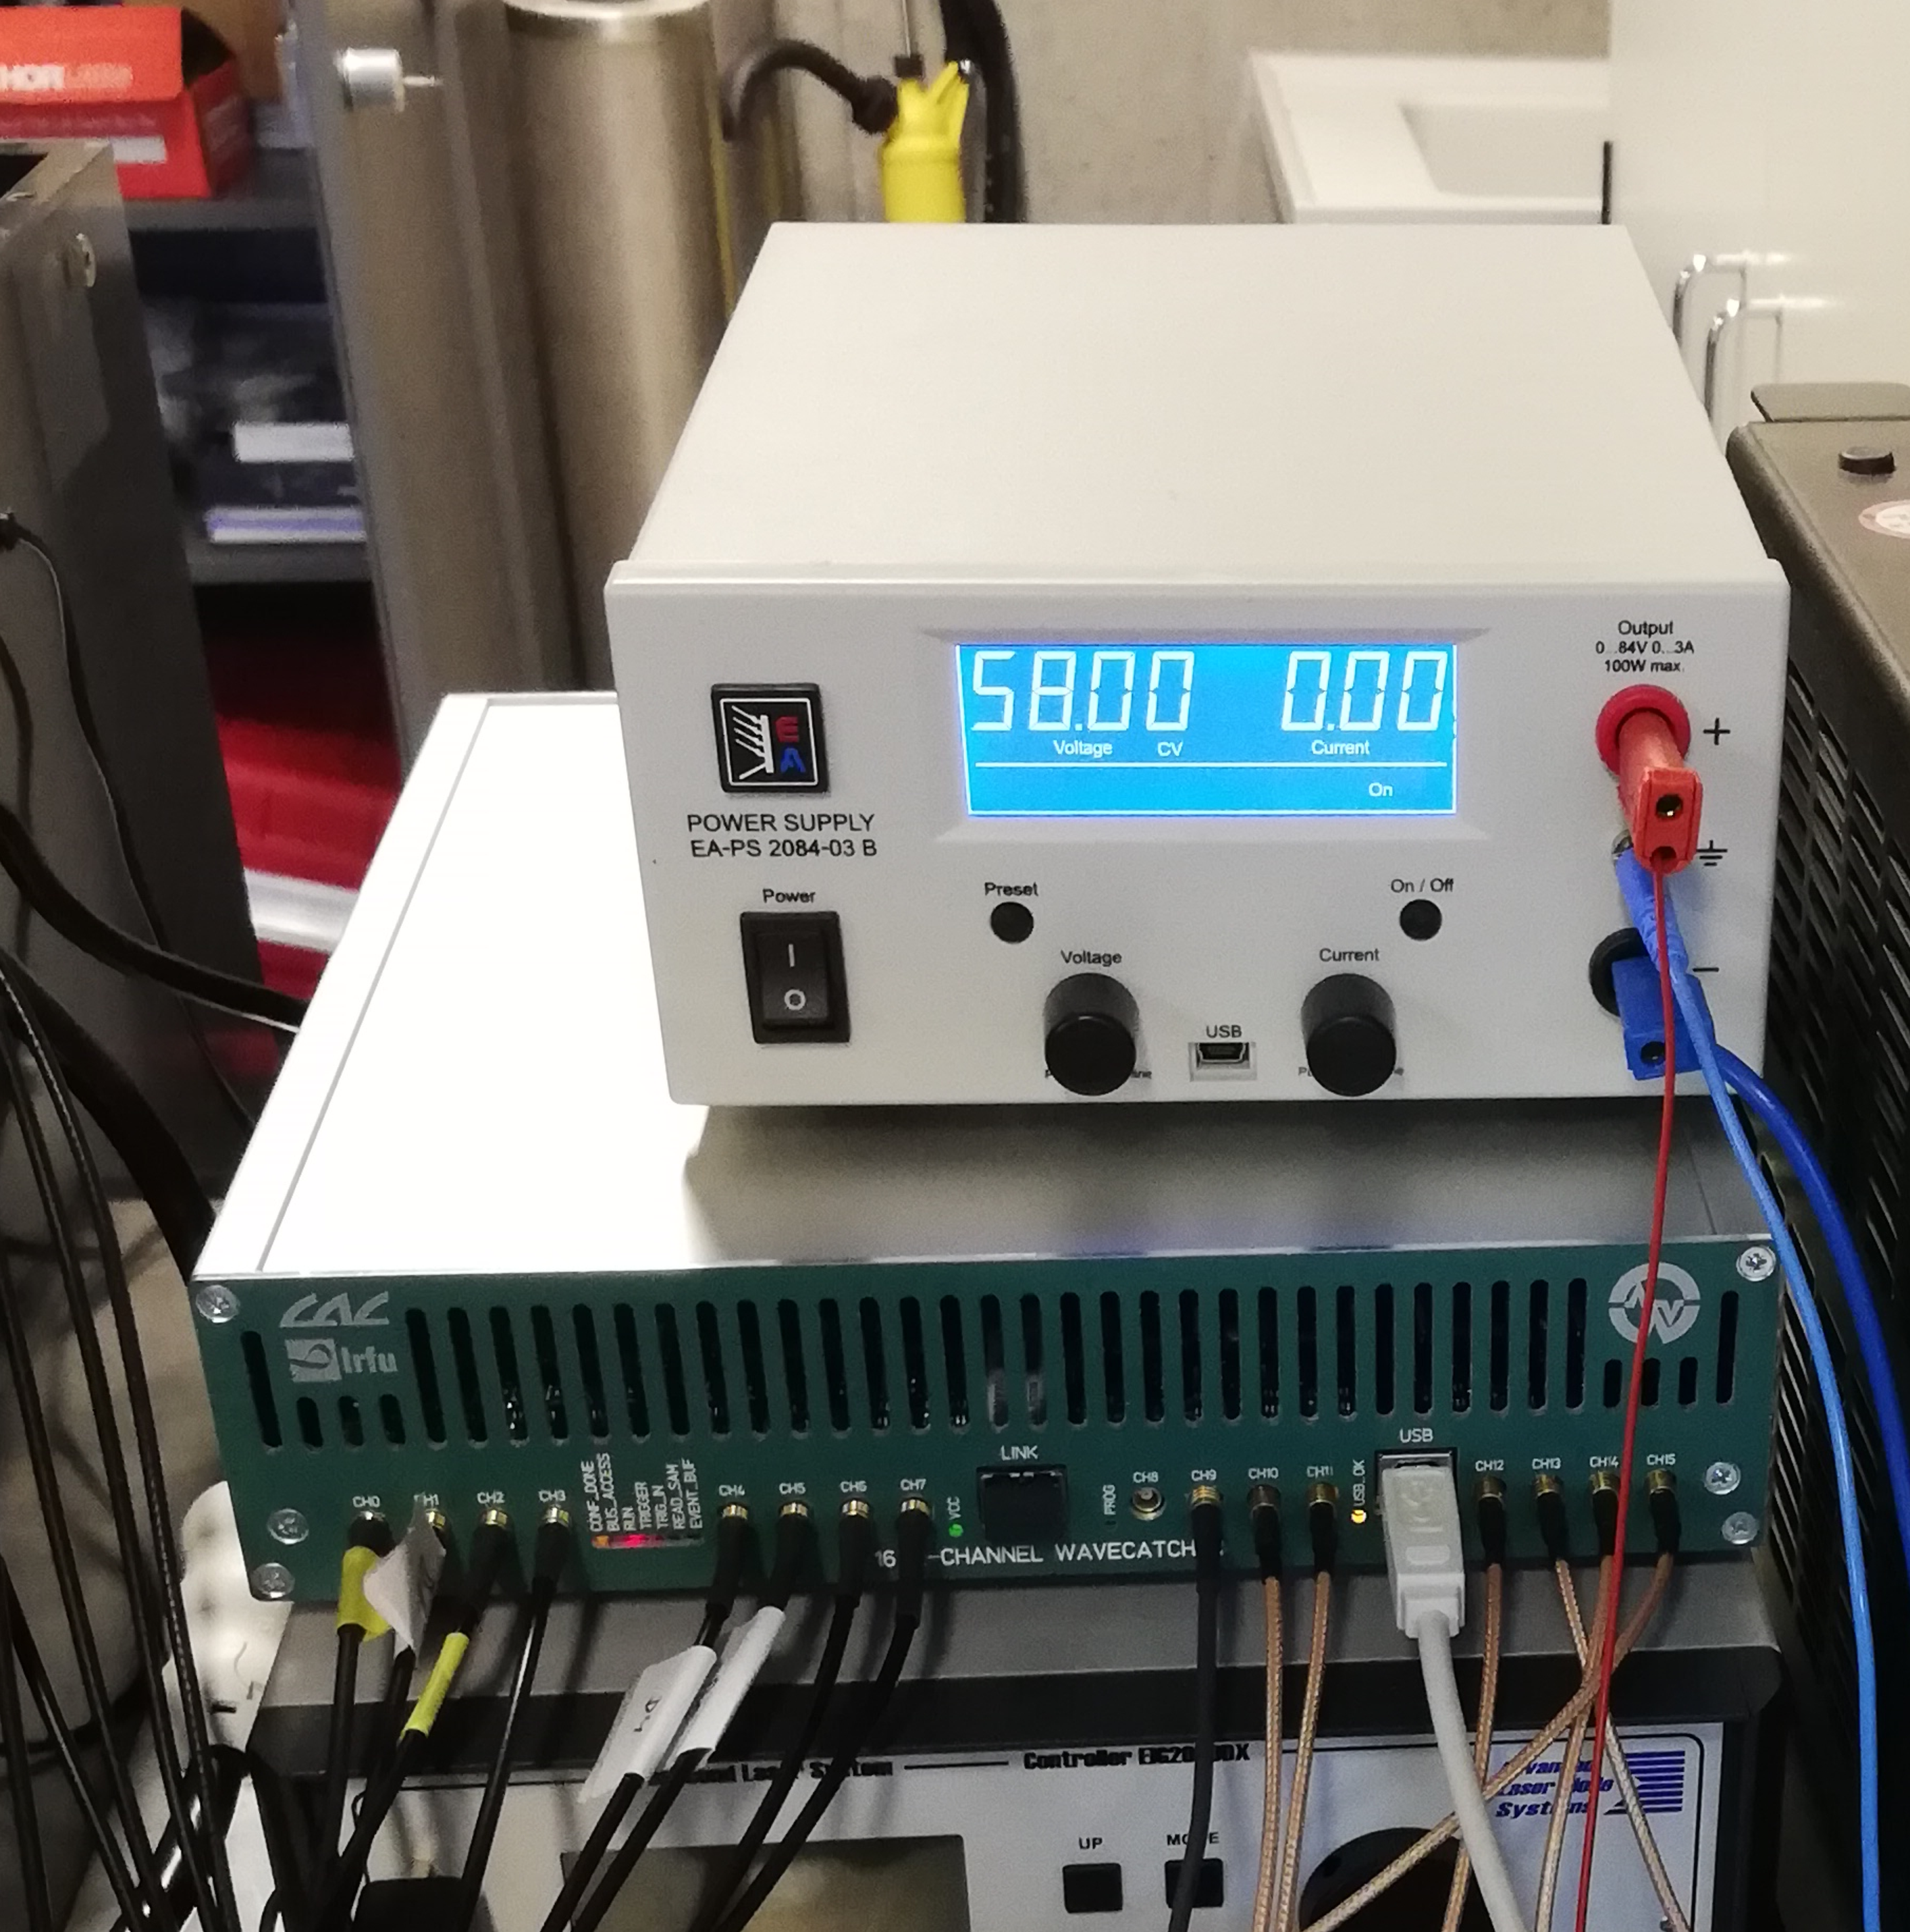
\includegraphics[width=\textwidth]{pictures/wavecatcher.pdf}
		\caption{}
	\end{subfigure}
	\caption{a) The eMUSIC board mounted to the PCB on top of the detector box. b) The WaveCatcher (green) and high voltage supply (white).}
	\label{fig:electronics}
\end{figure}

The eight amplified signals are then sent to a 16-channel WaveCatcher \cite{wavecatcher-manual} via an adapter board. The assignment of WaveCatcher channels to \ac{SiPM} groups is notated in table \ref{tab:channels}. The WaveCatcher acts as an analogue-to-digital converter, whose output is obtained via a USB-interface, connected to a computer running the appropriate software client \cite{wavecatcher-software}. 
This client is also used to configure the settings with which the experiment is run.

\begin{table}[h]
	\centering
	\begin{tabular}{@{}lll@{}}
		\midrule
		WaveCatcher channel  & Detector \\
		\midrule
		0-7          &   \ac{SiPM} groups 0-7 \\
		8, 9, 10, 11          &   \acsp{PMT} 1, 2, 3, 4\\
		12-15          &   unused\\
		\midrule
	\end{tabular}
	\caption{WaveCatcher channel assignment.}
	\label{tab:channels}
\end{table}

To trigger a muon event, the plastic scintillator and respective \ac{PMT} signals are used. The \acsp{PMT} are also connected to the WaveCatcher, in which the exact trigger requirements can be configured. In this experiment, the WaveCatcher records a \SI{320}{\nano\second} interval of data, if each of the four \acsp{PMT} experiences a voltage drop of at least \SI{4}{\milli\volt}, all in the span of \SI{15}{\nano\second}. This time interval is big enough that scintillation light generated by a crossing muon reaches the \acsp{PMT} on either side of both the plastic scintillators.

%\todo{irgendwie will er noch klarer detektor response zu muon event location haben}

\section{The Position-dependent Detector Response}

	The purpose of the \ac{SBT} will be to identify and locate muons around the decay vessel of the \ac{SHiP} experiment. For this, it is necessary to understand, how the \ac{SBT} responds to muons crossing it in different locations. As the \ac{SBT} will be composed of $\order{2000}$ individual detector cells, the study of this position-dependent detector response is done on prototypes of these cells.
	The prototype cell used in this thesis is made up of a steel box containing liquid scintillator, a \ac{WOM} tube inside a \ac{PMMA} vessel, both inserted into the \ac{LS} box, and, optically coupled to the \ac{WOM}, a ring-array of \num{40} \acsp{SiPM}. A muon crossing the \ac{LS} generates scintillation light in it, which, when reaching the \ac{WOM} gets wavelength-shifted from ultraviolet to visible light. These wavelength-shifted photons now travel inside the \ac{WOM} tube, total reflected off its walls, until they reach the end of the tube, where the \ac{SiPM} array is located. The \num{40} \acsp{SiPM} are readout in groups of 5, meaning 8 signals are recorded per muon-event. 
	It is now the goal to understand where the muon initially crossed the detector box (and generated scintillation light), solely from the 8 signals recorded from the \ac{SiPM} array. This is non-trivial, as the light generated in the scintillation will not reach the \ac{SiPM} directly, but first get reflected off the detector box' walls, and then wavelength-shifted. The latter process is non-directional, meaning the shifted photons get emitted into the \ac{WOM} tube isotropically, and reach the \ac{SiPM} array after travelling an arbitrarily complicated path inside the \ac{WOM} tube. This was illustrated in figure \ref{fig:travel-path}. Here, an exaggerated and simplified case was drawn to illustrate how the different responses of the \ac{SiPM} groups (numbered 0 to 7) show different amounts of light reaching them. 
	
	\begin{figure}
		\centering
		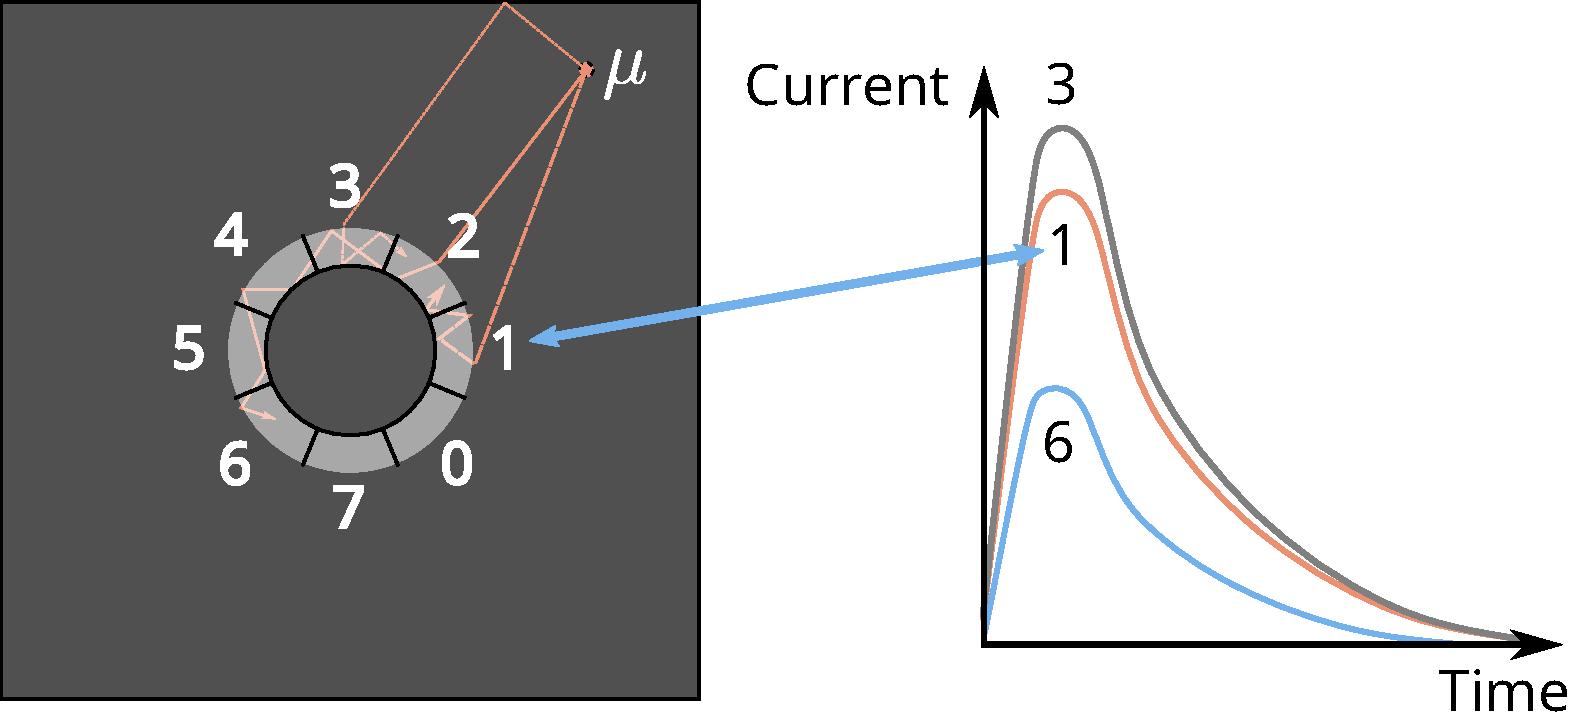
\includegraphics[width=.8\textwidth]{pictures/detector-response.pdf}
		\caption{Simplified illustration of a possible detector response. The left-hand picture shows a detector schematic, the right-hand side a simple current-time diagram of three \ac{SiPM} groups' signals. A muon $\mu$ crosses the detector box (dark grey), generating scintillation light (orange). The scintillation light reaches the \ac{WOM} with the mounted \ac{SiPM} channels 0-7 (light grey). Inside the \ac{WOM} the now shifted light travels until it reaches the end of the tube, where the \ac{SiPM} array is located. Not all \acsp{SiPM} 'see' the same amount of light, as illustrated in the diagram on the right-hand side - channels lying on 'opposite' sides of the muon event will also detect light, as the light inside the \ac{WOM} tube can travel in spirals.}
		\label{fig:travel-path}
	\end{figure}
	
	
	
	To understand the position-dependent response of the detector prototype, the cosmics setup uses cosmics muons, triggered by a set of two plastic scintillators, to study the behaviour of the prototype for different muon-crossing locations. The determination of this location is possible with the plastic scintillators, which are located above and beneath the detector box, and readout with a set of two \ac{PMT} each. Considering only certain muon-crossing positions, the signals measured in the prototype were now analysed and compared.
	The next chapter explains how the \ac{SiPM} groups' signals were interpreted, and how the plastic scintillators were used to determine a muon's crossing position.
	





